
% figure of traffic network

  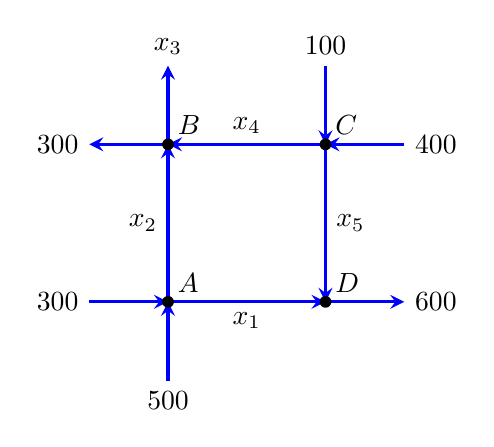
\begin{tikzpicture}
    \coordinate (A) at (-1,-1); \node[anchor=south west] at (A) {$A$};
    \coordinate (B) at (-1,1); \node[anchor=south west] at (B) {$B$};
    \coordinate (C) at (1,1); \node[anchor=south west] at (C) {$C$};
    \coordinate (D) at (1,-1); \node[anchor=south west] at (D) {$D$};
    \draw[very thick,blue,stealth-] (A)--node[pos=1,anchor=north,black] () {$500$} ++(0,-1);
    \draw[very thick,blue,stealth-] (A)--node[pos=1,anchor=east,black] () {$300$} ++(-1,0);
    \draw[very thick,blue,-stealth] (B)--node[pos=1,anchor=east,black] () {$300$} ++(-1,0);
    \draw[very thick,blue,-stealth] (B)--node[pos=1,anchor=south,black] () {$x_3$} ++(0,1);
    \draw[very thick,blue,stealth-] (C)--node[pos=1,anchor=south,black] () {$100$} ++(0,1);
    \draw[very thick,blue,stealth-] (C)--node[pos=1,anchor=west,black] () {$400$} ++(1,0);
    \draw[very thick,blue,-stealth] (D)--node[pos=1,anchor=west,black] () {$600$} ++(1,0);
    \draw[very thick,blue,-stealth] (A)--node[pos=.5,anchor=east,black] () {$x_2$} (B);
    \draw[very thick,blue,-stealth] (C)--node[pos=.5,anchor=south,black] () {$x_4$} (B);
    \draw[very thick,blue,-stealth] (A)--node[pos=.5,anchor=north,black] () {$x_1$} (D);
    \draw[very thick,blue,-stealth] (C)--node[pos=.5,anchor=west,black] () {$x_5$} (D);
    \node[circle,fill,inner sep=1.5pt] at (A) {};
    \node[circle,fill,inner sep=1.5pt] at (B) {};
    \node[circle,fill,inner sep=1.5pt] at (C) {};
    \node[circle,fill,inner sep=1.5pt] at (D) {};
  \end{tikzpicture}
